\chapter{Binary Relations, Mappings \& Abstract Algebraic Structures}
\label{chap:relations_structures}

\section{Binary Relations and Equivalence Structures}

\begin{definitionbox}{Binary Relation and Fundamental Axiomatic Properties}
Let $E$ be a set. A \textbf{binary relation} $\mathcal{R}$ on $E$ is formally defined as a subset of the Cartesian product: $\mathcal{R} \subseteq E \times E$. We write $x \mathcal{R} y$ if and only if $(x, y) \in \mathcal{R}$.
\begin{enumerate}[leftmargin=1.4em,itemsep=3pt]
  \item \textbf{Reflexivity:} $\forall x \in E, \ x \mathcal{R} x$.
  \item \textbf{Symmetry:} $\forall x, y \in E, \ (x \mathcal{R} y \implies y \mathcal{R} x)$.
  \item \textbf{Antisymmetry:} $\forall x, y \in E, \ ((x \mathcal{R} y \land y \mathcal{R} x) \implies x = y)$.
  \item \textbf{Transitivity:} $\forall x, y, z \in E, \ ((x \mathcal{R} y \land y \mathcal{R} z) \implies x \mathcal{R} z)$.
\end{enumerate}
\end{definitionbox}

\begin{definitionbox}{Equivalence Relations and Quotient Sets}
A binary relation $\mathcal{R}$ is an \textbf{equivalence relation} if it is simultaneously \textbf{reflexive, symmetric, and transitive}.
\begin{enumerate}[leftmargin=1.4em,itemsep=2pt]
  \item The \textbf{equivalence class} of an element $x \in E$ is the set of all elements related to $x$:
  \[
  \mathrm{cl}(x) \equiv [x] = \{ y \in E \mid x \mathcal{R} y \}.
  \]
  \item The \textbf{quotient set} $E / \mathcal{R}$ is the set of all distinct equivalence classes:
  \[
  E / \mathcal{R} = \{ [x] \mid x \in E \}.
  \]
\end{enumerate}
\end{definitionbox}

\begin{theorembox}{Fundamental Theorem of Equivalence Relations (Partition Theorem)}
Let $\mathcal{R}$ be an equivalence relation on $E$.
\begin{enumerate}[leftmargin=1.4em,itemsep=2pt]
  \item Two equivalence classes are either identical or completely disjoint:
  \[
  \forall x, y \in E, \quad [x] = [y] \iff x \mathcal{R} y, \qquad [x] \cap [y] = \emptyset \iff \neg(x \mathcal{R} y).
  \]
  \item The quotient set $E / \mathcal{R}$ forms a \textbf{partition} of $E$: the classes are non-empty, pairwise disjoint, and their union recovers $E$:
  \[
  \bigcup_{[x] \in E/\mathcal{R}} [x] = E.
  \]
\end{enumerate}
\end{theorembox}

\section{Order Relations and Posets}

\begin{definitionbox}{Partial and Total Orders}
A binary relation $\le$ on $E$ is an \textbf{order relation} if it is \textbf{reflexive, antisymmetric, and transitive}. The pair $(E, \le)$ is called a \textbf{partially ordered set} (or \textit{poset}).
\begin{itemize}[leftmargin=1.4em,itemsep=2pt]
  \item \textbf{Total Order (Chain):} If every pair of elements is comparable:
  \[
  \forall x, y \in E, \quad (x \le y \lor y \le x).
  \]
  \item \textbf{Partial Order:} There exist elements $x, y \in E$ such that neither $x \le y$ nor $y \le x$ (e.g. set inclusion $\subseteq$ on $\mathcal{P}(E)$).
\end{itemize}
\end{definitionbox}

\section{Mappings, Functions, and Morphisms}

\begin{figure}[htbp]
  \centering
  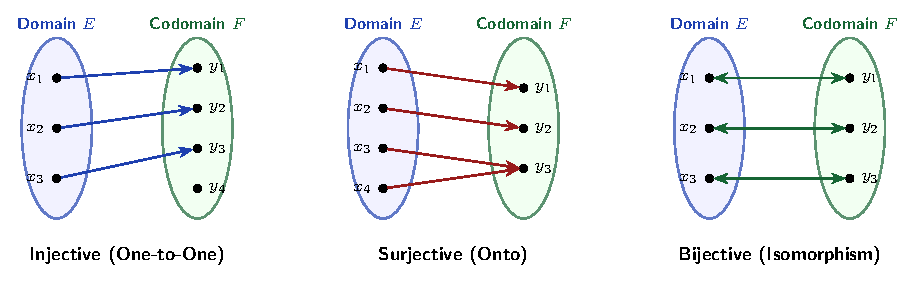
\includegraphics[width=0.95\textwidth]{02_mapping_types.pdf}
  \caption{\textbf{Classification of Mappings:} Injective (each codomain element has at most one preimage), Surjective (every codomain element has at least one preimage), and Bijective (exact one-to-one correspondence).}
  \label{fig:mappings}
\end{figure}

\begin{definitionbox}{Injectivity, Surjectivity, and Bijectivity}
Let $f: E \longrightarrow F$ be a mapping from set $E$ to set $F$:
\begin{enumerate}[leftmargin=1.4em,itemsep=3pt]
  \item \textbf{Injective (One-to-One):} Distinct domain elements map to distinct images:
  \[
  \forall x_1, x_2 \in E, \quad \left( f(x_1) = f(x_2) \implies x_1 = x_2 \right) \iff \left( x_1 \neq x_2 \implies f(x_1) \neq f(x_2) \right).
  \]
  \item \textbf{Surjective (Onto):} Every element of the codomain is the image of at least one domain element:
  \[
  \forall y \in F, \quad \exists x \in E \ \text{such that} \ f(x) = y \iff f(E) = F.
  \]
  \item \textbf{Bijective:} $f$ is both injective and surjective.
  Equivalently, for every $y \in F$, the equation $f(x) = y$ has a \textbf{unique solution} $x \in E$:
  \[
  \forall y \in F, \quad \exists! x \in E, \quad f(x) = y.
  \]
  A mapping $f$ is bijective if and only if there exists an inverse mapping $f^{-1}: F \longrightarrow E$ satisfying:
  \[
  f^{-1} \circ f = \mathrm{id}_E \quad \text{and} \quad f \circ f^{-1} = \mathrm{id}_F.
  \]
\end{enumerate}
\end{definitionbox}

\begin{propbox}{Properties of Image and Preimage Sets}
Let $f: E \longrightarrow F$. For any subsets $A, A' \subseteq E$ and $B, B' \subseteq F$:
\begin{enumerate}[leftmargin=1.4em,itemsep=2pt]
  \item $f(A \cup A') = f(A) \cup f(A')$ and $f(A \cap A') \subseteq f(A) \cap f(A')$ (equality holds if $f$ is injective).
  \item $f^{-1}(B \cup B') = f^{-1}(B) \cup f^{-1}(B')$ and $f^{-1}(B \cap B') = f^{-1}(B) \cap f^{-1}(B')$.
  \item $f^{-1}(\complement_F B) = \complement_E (f^{-1}(B))$. (Preimages preserve all boolean operations!).
\end{enumerate}
\end{propbox}

\section{Abstract Algebraic Structures}

\begin{figure}[htbp]
  \centering
  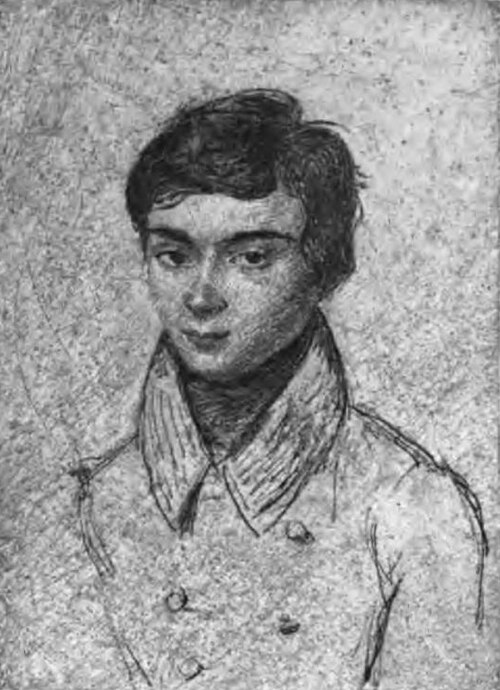
\includegraphics[width=0.28\textwidth]{galois.jpg}
  \caption{\textbf{Évariste Galois (1811--1832)}, French mathematical genius who introduced the concept of a \textit{group} and symmetry permutations to resolve the unsolvability of general quintic polynomial equations by radicals.}
  \label{fig:galois}
\end{figure}

\begin{definitionbox}{Groups, Subgroups, and Homomorphisms}
An \textbf{internal binary operation} on a set $G$ is a mapping $*: G \times G \longrightarrow G, (x, y) \mapsto x * y$.
\begin{enumerate}[leftmargin=1.4em,itemsep=3pt]
  \item A pair $(G, *)$ is a \textbf{Group} if:
  \begin{itemize}[leftmargin=1.2em,itemsep=1pt]
    \item \textbf{Associativity:} $\forall x, y, z \in G, \ (x * y) * z = x * (y * z)$.
    \item \textbf{Neutral Element:} $\exists e \in G, \ \forall x \in G, \ x * e = e * x = x$.
    \item \textbf{Invertibility:} $\forall x \in G, \ \exists x' \in G, \ x * x' = x' * x = e$ (denoted $x^{-1}$).
  \end{itemize}
  If additionally $\forall x, y \in G, x * y = y * x$, the group is \textbf{Abelian} (or commutative).
  \item \textbf{Subgroup Criterion:} A non-empty subset $H \subseteq G$ is a subgroup ($H \le G$) if and only if:
  \[
  \forall x, y \in H, \quad x * y^{-1} \in H.
  \]
  \item \textbf{Group Homomorphism:} A mapping $\phi: (G, *) \longrightarrow (G', \star)$ such that:
  \[
  \forall x, y \in G, \quad \phi(x * y) = \phi(x) \star \phi(y).
  \]
  The \textbf{kernel} $\ker(\phi) = \{ x \in G \mid \phi(x) = e' \}$ is a normal subgroup of $G$, and $\phi$ is injective if and only if $\ker(\phi) = \{ e \}$.
\end{enumerate}
\end{definitionbox}

\begin{definitionbox}{Rings and Fields}
\begin{enumerate}[leftmargin=1.4em,itemsep=3pt]
  \item A triplet $(A, +, \cdot)$ is a \textbf{Ring} if $(A, +)$ is an abelian group (neutral $0$), the operation $\cdot$ is associative, and $\cdot$ distributes over $+$:
  \[
  \forall x, y, z \in A, \quad x \cdot (y + z) = x \cdot y + x \cdot z \quad \text{and} \quad (y + z) \cdot x = y \cdot x + z \cdot x.
  \]
  \item A ring $(K, +, \cdot)$ is a \textbf{Field} (Corps) if $0 \neq 1$, multiplication is commutative, and every non-zero element $x \in K \setminus \{0\}$ has a multiplicative inverse $x^{-1}$.
  (\textit{Examples:} $\mathbb{Q}, \mathbb{R}, \mathbb{C}$ are fields; $\mathbb{Z}$ is an integral domain but not a field).
\end{enumerate}
\end{definitionbox}

\section{Worked Examples with Step-by-Step Proofs}

\begin{workedexample}{Modular Arithmetic as an Equivalence Relation}
Fix an integer $n \ge 2$. On the set of integers $\mathbb{Z}$, define the relation of \textbf{congruence modulo $n$} by:
\[
x \equiv y \pmod n \iff n \mid (x - y) \iff \exists k \in \mathbb{Z}, \ x - y = k n.
\]
\begin{enumerate}[leftmargin=1.4em,itemsep=2pt]
  \item Prove rigorously that $\equiv \pmod n$ is an equivalence relation on $\mathbb{Z}$.
  \item Describe explicitly the equivalence classes and the quotient set $\mathbb{Z} / n\mathbb{Z}$.
\end{enumerate}

\paragraph{Solution and Proof.}
\textbf{1. Verification of Equivalence Axioms:}
\begin{itemize}[leftmargin=1.4em,itemsep=2pt]
  \item \textbf{Reflexivity:} For any $x \in \mathbb{Z}$, $x - x = 0 = 0 \cdot n$. Since $0 \in \mathbb{Z}$, $n \mid (x - x)$, so $x \equiv x \pmod n$.
  \item \textbf{Symmetry:} Let $x, y \in \mathbb{Z}$ such that $x \equiv y \pmod n$.
  Then $x - y = k n$ for some $k \in \mathbb{Z}$. Multiplying by $-1$:
  \[
  y - x = -(x - y) = -k n = (-k) n.
  \]
  Since $-k \in \mathbb{Z}$, $n \mid (y - x)$, so $y \equiv x \pmod n$.
  \item \textbf{Transitivity:} Let $x, y, z \in \mathbb{Z}$ such that $x \equiv y \pmod n$ and $y \equiv z \pmod n$.
  Then $x - y = k_1 n$ and $y - z = k_2 n$ for integers $k_1, k_2 \in \mathbb{Z}$.
  Adding the two equations:
  \[
  (x - y) + (y - z) = k_1 n + k_2 n \implies x - z = (k_1 + k_2) n.
  \]
  Since $k_1 + k_2 \in \mathbb{Z}$, $n \mid (x - z)$, so $x \equiv z \pmod n$.
\end{itemize}
Therefore, $\equiv \pmod n$ is an equivalence relation.

\textbf{2. Equivalence Classes and Quotient Set:}
By the Euclidean division algorithm, for any integer $x \in \mathbb{Z}$, dividing by $n$ yields unique integers $q \in \mathbb{Z}$ and $r \in \{0, 1, 2, \dots, n-1\}$ such that:
\[
x = q n + r \implies x - r = q n \implies x \equiv r \pmod n.
\]
Hence, every integer belongs to the equivalence class of its remainder $r \in \{0, 1, \dots, n-1\}$:
\[
[r] = \{ r + k n \mid k \in \mathbb{Z} \} = r + n\mathbb{Z}.
\]
The quotient set consists of exactly $n$ distinct equivalence classes:
\[
\mathbf{\mathbb{Z} / n\mathbb{Z} = \{ [0], [1], [2], \dots, [n-1] \}}. \quad \blacksquare
\]
\end{workedexample}

\begin{workedexample}{Injectivity, Surjectivity, and Bijectivity Verification}
Consider the mapping:
\[
f: \mathbb{R} \setminus \{2\} \longrightarrow \mathbb{R} \setminus \{1\}, \qquad f(x) = \frac{x + 1}{x - 2}.
\]
\begin{enumerate}[leftmargin=1.4em,itemsep=2pt]
  \item Prove from first principles that $f$ is injective.
  \item Prove from first principles that $f$ is surjective.
  \item Deduce that $f$ is bijective and determine its explicit inverse mapping $f^{-1}(y)$.
\end{enumerate}

\paragraph{Solution and Proof.}
\textbf{1. Proof of Injectivity:}
Let $x_1, x_2 \in \mathbb{R} \setminus \{2\}$ such that $f(x_1) = f(x_2)$:
\[
\frac{x_1 + 1}{x_1 - 2} = \frac{x_2 + 1}{x_2 - 2}.
\]
Cross-multiplying denominators:
\[
(x_1 + 1)(x_2 - 2) = (x_2 + 1)(x_1 - 2).
\]
Expanding both products:
\[
x_1 x_2 - 2 x_1 + x_2 - 2 = x_1 x_2 - 2 x_2 + x_1 - 2.
\]
Subtracting the common terms $x_1 x_2 - 2$ from both sides:
\[
-2 x_1 + x_2 = -2 x_2 + x_1 \implies 3 x_2 = 3 x_1 \implies x_1 = x_2.
\]
Thus $f$ is strictly \textbf{injective}.

\textbf{2. Proof of Surjectivity:}
Let $y \in \mathbb{R} \setminus \{1\}$ be an arbitrary element of the codomain. We must find $x \in \mathbb{R} \setminus \{2\}$ such that $f(x) = y$:
\[
\frac{x + 1}{x - 2} = y \implies x + 1 = y(x - 2) = y x - 2y.
\]
Isolating terms in $x$:
\[
1 + 2y = y x - x = x(y - 1).
\]
Since $y \neq 1$, we can divide by $(y - 1) \neq 0$:
\[
x = \frac{2y + 1}{y - 1}.
\]
We must verify that this candidate $x \neq 2$:
If $\frac{2y+1}{y-1} = 2 \implies 2y + 1 = 2y - 2 \implies 1 = -2$, which is impossible.
Hence $x \in \mathbb{R} \setminus \{2\}$ always exists and is well-defined.
Thus $f$ is \textbf{surjective}.

\textbf{3. Bijectivity and Inverse Mapping:}
Since $f$ is both injective and surjective, it is a \textbf{bijection}.
Its inverse mapping $f^{-1}: \mathbb{R} \setminus \{1\} \longrightarrow \mathbb{R} \setminus \{2\}$ is:
\[
\mathbf{f^{-1}(y) = \frac{2y + 1}{y - 1}}. \quad \blacksquare
\]
\end{workedexample}

\begin{workedexample}{Subgroup Verification and Matrix Groups}
Let $\mathrm{GL}_2(\mathbb{R})$ denote the general linear group of $2 \times 2$ invertible real matrices under matrix multiplication. Consider the subset:
\[
\mathrm{SL}_2(\mathbb{R}) = \{ M \in \mathrm{GL}_2(\mathbb{R}) \mid \det(M) = 1 \}.
\]
Prove using the subgroup criterion that $\mathrm{SL}_2(\mathbb{R})$ is a subgroup of $\mathrm{GL}_2(\mathbb{R})$ (the \textit{Special Linear Group}).

\paragraph{Solution and Proof.}
We verify the three conditions of the subgroup criterion:
\begin{enumerate}[leftmargin=1.4em,itemsep=3pt]
  \item \textbf{Non-emptiness:}
  The identity matrix $I_2 = \begin{pmatrix} 1 & 0 \\ 0 & 1 \end{pmatrix}$ has determinant:
  \[
  \det(I_2) = (1)(1) - (0)(0) = 1.
  \]
  Thus $I_2 \in \mathrm{SL}_2(\mathbb{R})$, establishing that $\mathrm{SL}_2(\mathbb{R}) \neq \emptyset$.
  \item \textbf{Closure under Inverse:}
  Let $A \in \mathrm{SL}_2(\mathbb{R})$. Then $\det(A) = 1 \neq 0$, so $A^{-1}$ exists in $\mathrm{GL}_2(\mathbb{R})$.
  By the multiplicative property of determinants:
  \[
  \det(A \cdot A^{-1}) = \det(I_2) = 1 \implies \det(A) \cdot \det(A^{-1}) = 1.
  \]
  Since $\det(A) = 1$, we have $1 \cdot \det(A^{-1}) = 1 \implies \det(A^{-1}) = 1$.
  Therefore, $A^{-1} \in \mathrm{SL}_2(\mathbb{R})$.
  \item \textbf{Closure under Product (Combined Criterion $A B^{-1} \in \mathrm{SL}_2(\mathbb{R})$):}
  Let $A, B \in \mathrm{SL}_2(\mathbb{R})$.
  \[
  \det(A B^{-1}) = \det(A) \cdot \det(B^{-1}) = 1 \times 1 = 1.
  \]
  Therefore, $A B^{-1} \in \mathrm{SL}_2(\mathbb{R})$.
\end{enumerate}
By the Subgroup Criterion, $\mathbf{\mathrm{SL}_2(\mathbb{R}) \le \mathrm{GL}_2(\mathbb{R})}$ is a subgroup. $\blacksquare$
\end{workedexample}

\begin{workedexample}{Kernel and Image of a Group Homomorphism}
Consider the mapping $\phi: (\mathbb{R}, +) \longrightarrow (\mathbb{C}^*, \cdot)$ defined by:
\[
\phi(x) = e^{i x} = \cos(x) + i \sin(x).
\]
\begin{enumerate}[leftmargin=1.4em,itemsep=2pt]
  \item Prove that $\phi$ is a group homomorphism.
  \item Determine the kernel $\ker(\phi)$ and describe its algebraic nature.
  \item Determine the image $\mathrm{Im}(\phi)$.
\end{enumerate}

\paragraph{Solution and Proof.}
\textbf{1. Proof of Homomorphism:}
For any $x, y \in \mathbb{R}$:
\[
\phi(x + y) = e^{i(x + y)} = e^{i x} \cdot e^{i y} = \phi(x) \cdot \phi(y).
\]
Since addition in the domain maps to multiplication in the codomain, $\phi$ is a group homomorphism.

\textbf{2. Kernel Determination:}
The neutral element of $(\mathbb{C}^*, \cdot)$ is $1$. By definition:
\[
\ker(\phi) = \{ x \in \mathbb{R} \mid \phi(x) = 1 \} = \{ x \in \mathbb{R} \mid \cos x + i \sin x = 1 \}.
\]
Equating real and imaginary parts:
\[
\cos x = 1 \quad \text{and} \quad \sin x = 0 \iff x = 2 k \pi \quad (k \in \mathbb{Z}).
\]
Therefore:
\[
\mathbf{\ker(\phi) = 2\pi\mathbb{Z} = \{ 2 k \pi \mid k \in \mathbb{Z} \}}.
\]
Notice that $\ker(\phi) \neq \{0\}$, proving that $\phi$ is \textbf{not injective}.

\textbf{3. Image Determination:}
For every $x \in \mathbb{R}$, $|\phi(x)| = |e^{i x}| = \sqrt{\cos^2 x + \sin^2 x} = 1$.
Every complex number on the unit circle $\mathbb{U} = \{ z \in \mathbb{C} \mid |z| = 1 \}$ can be written in polar form as $e^{i \theta}$ for some $\theta \in \mathbb{R}$.
Therefore:
\[
\mathbf{\mathrm{Im}(\phi) = \mathbb{U} \equiv \mathbb{S}^1} \quad \text{(the Circle Group)}. \quad \blacksquare
\]
\end{workedexample}
